% !TEX root = Master.tex

\textbf{Sparse Data Case}\\
As mentioned before, at the beginning of this study the availability of attributes in the LiDAR dataset was limited to just the height and location of the detected trees. A problem, as only regression models using those parameters could be included. Expert knowledge and further research highly advised using tree species and potentially the crown-area. \\

Consequently, the entire forest must be rearranged in such a way that sections with a similar structure are clustered together. The clustering of the sections can be highly advantageous. Important information of variables can be explained by the clusters. For example, there might be two areas with different dominant tree species. Those two species differ significantly in height and diameter. Clustering based on some variables could then detect those areas to be different and thus separate them.\\

Subsequently, for each cluster of multiple sections a regression model is created and later applied on the LiDAR data, resulting in better predictions. \\

To cluster sections, each of them requires numerical values. As discussed, the height and diameter are intuitive variables which can be used. Thus, the mean and variance for both variables are calculated for each tree in the individual sections and then assigned to them, allowing to apply common clustering methods.\\

In conclusion, each section four variables are assigned describing the structure of its tree (mean diameter, mean height, variance diameter, variance height). They are then clustered with the goal that subsequent regression models describe as much variation as if important variables (tree species, crown area) would exist.\\

We compared k-means and hierarchical clustering (single \& complete linkage). Hierarchical methods group two data points iteratively, until one cluster containing all observations exist. A group is built with two variables which have the minimal distance compared to all other data points. After grouping one pair, the distance from each variable to the newly grouped variables is calculated and the next grouping step begins. The distance can be calculated with different linkage methods. Minimum distance for single linkage and maximum distance for complete linkage was compared.\\

Hierarchical clustering will therefore group outliers at the very end, resulting in several clusters with only one section (outlier). This is undesirable, as one should consider that the auxiliary variables used for clustering are based on few samples. Applying regression models on sparse sections will likely lead to overfitting. Thus, hierarchical clustering is discarded.

\begin{figure}[H]
\centering
  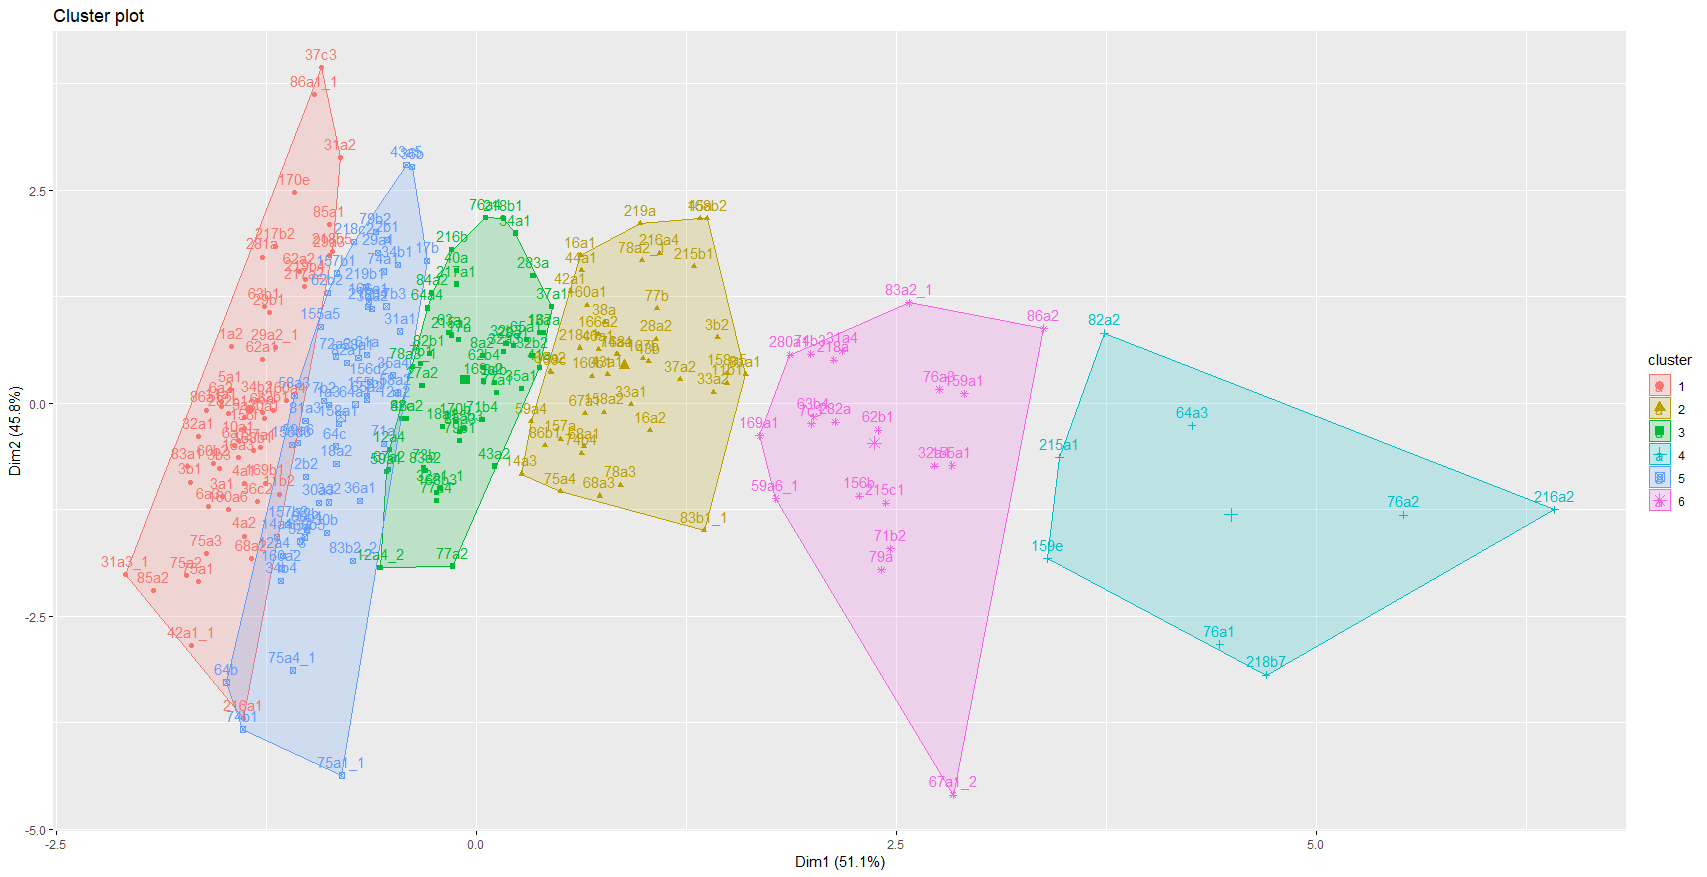
\includegraphics[scale = 0.85]{appendix_cluster.png}
  \caption{Clustered sections with respect to mean and variance of both height and diameter using principal components.}
  \label{fig:appendix_cluster}
\end{figure}

Figure \ref{fig:appendix_cluster} provides a visual representation using the first two Principle Components and then draw an ellipse around each cluster (using R package factoextra[8]). 

\begin{figure}[H]
\centering
  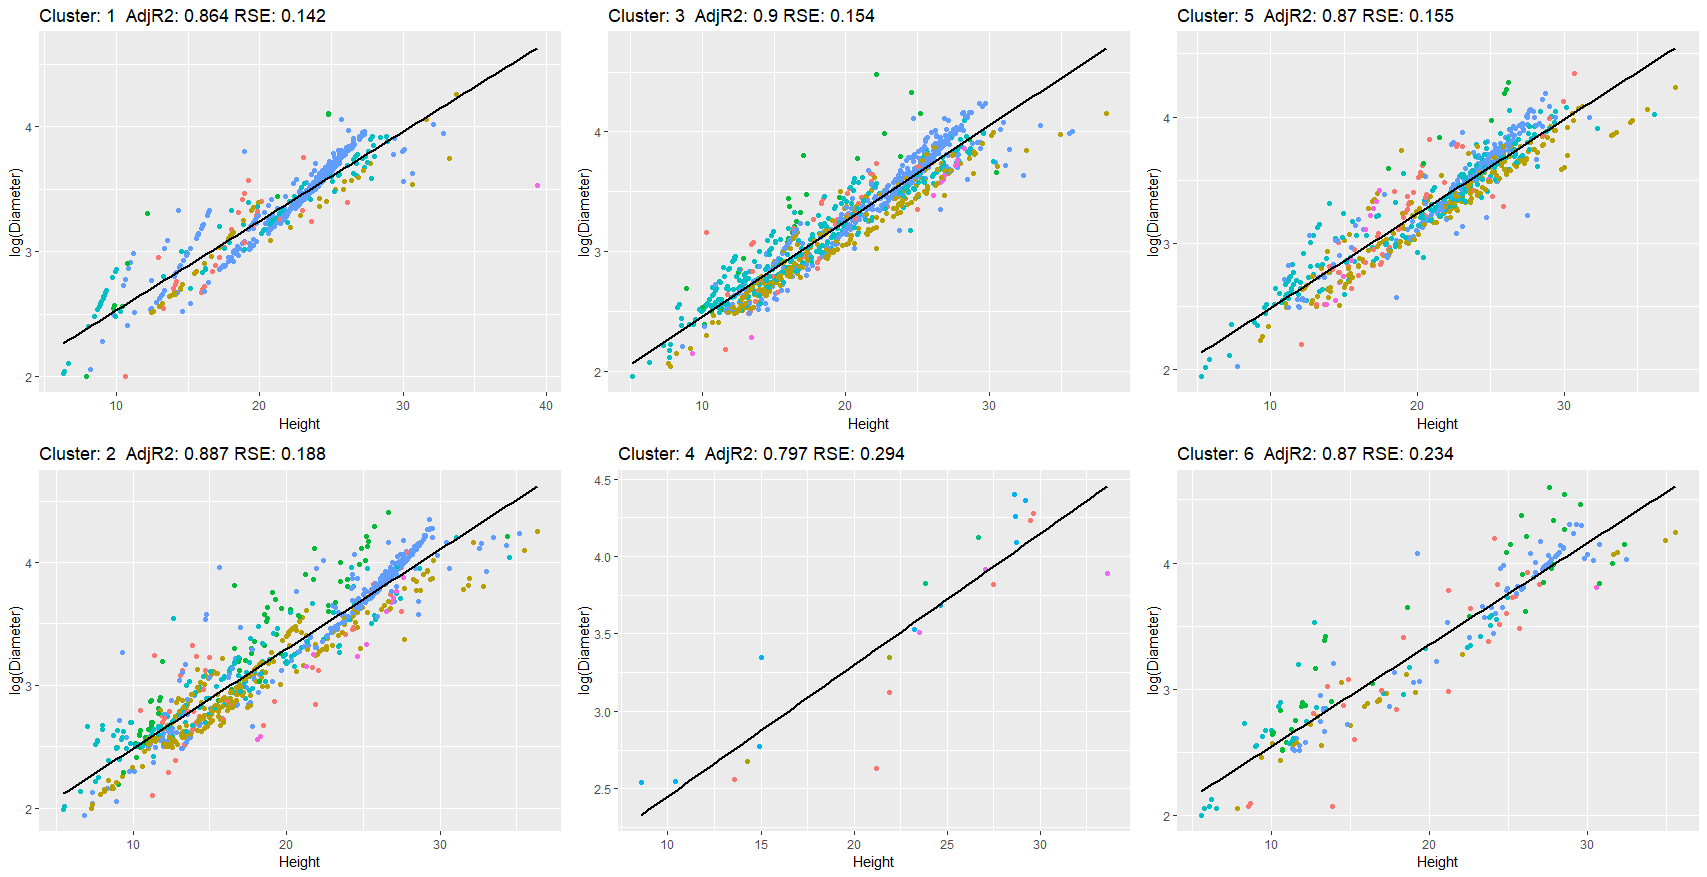
\includegraphics[scale = 0.85]{multi_regression.png}
  \caption{: Log-linear regression models log(diameter) \textasciitilde height for each cluster. The color indicates the tree species.}
  \label{fig:multi_regression}
\end{figure}



\begin{table}[H]
\centering
\setlength\arrayrulewidth{1pt}
\begin{adjustbox}{max width=\textwidth}

\begin{tabular}{|c|c|c|}
\hline 
\rowcolor{Gray}
\textbf{Cluster} & \textbf{Intercept} & \textbf{Height} \\ 
\hline 
1 & 1.7428 & 0.0745 \\ 
\hline 
2 & 1.6768 & 0.0808 \\ 
\hline 
3 & 1.5997 & 0.0849 \\ 
\hline 
4 & 1.6607 & 0.0795 \\ 
\hline 
5 & 1.7386 & 0.0805 \\ 
\hline 
6 & 1.8159 & 0.0713 \\ 
\hline 
\end{tabular} 

\end{adjustbox}

\caption{Estimates of the log-linear models based on k-means clustering}
\label{tab:appendix_table}
\end{table}

Regression models on each cluster showed satisfying results with adjusted R² around 0.87 for the largest cluster (see Figure \ref{fig:multi_regression}). After acquiring the additional information on crown area and species group, this approach was neglected. 
